% coding:utf-8

%FOSAET, a LaTeX-Code for a electrical summary of basic electronics
%TV-B-Gone
%Copyright (C) 2013, Daniel Winz, Ervin Mazlagic

%This program is free software; you can redistribute it and/or
%modify it under the terms of the GNU General Public License
%as published by the Free Software Foundation; either version 2
%of the License, or (at your option) any later version.

%This program is distributed in the hope that it will be useful,
%but WITHOUT ANY WARRANTY; without even the implied warranty of
%MERCHANTABILITY or FITNESS FOR A PARTICULAR PURPOSE.  See the
%GNU General Public License for more details.
%----------------------------------------

\documentclass[a4paper,
               10pt,
               fleqn]{article}

\author{Ervin Mazlagic}
\title{Paper Manual}
\title{TV-B-Gone}

\usepackage{luxpaper}
\usepackage{luxtitle}
 
\begin{document}
\luxtitle{Papers}
         {TV-B-Gone}
         {Ervin Mazlagi\'c, Daniel Winz}
         {Adligenswil}
         {2012}

\tableofcontents
\newpage

% coding:utf-8

%TV-B-Gone
%Copyright (C) 2013, Daniel Winz, Ervin Mazlagic

%This program is free software; you can redistribute it and/or
%modify it under the terms of the GNU General Public License
%as published by the Free Software Foundation; either version 2
%of the License, or (at your option) any later version.

%This program is distributed in the hope that it will be useful,
%but WITHOUT ANY WARRANTY; without even the implied warranty of
%MERCHANTABILITY or FITNESS FOR A PARTICULAR PURPOSE.  See the
%GNU General Public License for more details.
%----------------------------------------

\section{Einleitung}
Das Ziel dieses Projektes ist es, das ECAD Kicad und die Controllerfamilie 
MSP430 von Texas Instruments kennen zu lernen. 

Dazu wurde ein kleines Projekt gesucht, das sowohl Hardware als auch Firmware 
beinhaltet. Die Entscheidung fiel auf ein TV-B-Gone. Dies ist ein Gerät, das 
in der Lage ist, verschiedene Geräte via Infrarot (z.B. RC-5) auszuschalten. 

Zunächst werden Erfahrungen mit dem MSP430 gesammelt. Als Plattform dazu dient 
das Launchpad von Texas Instruments. 

\section{Code Konventionen}
Bei Code-Projekten aller Art ist es wichtig, dass alle Mitglieder gewissen
Style-Konventionen folgen (diese können selbst definiert werden und auch
entgegen allen Empfehlungen sein, jedoch sollten diese einmal aufgesetzt
auch gefolgt werden).

Als Orientierungshilfe kann beispielsweise das Paper von GNU\footnote{
    \emph{GNU coding standards} beschreibt Konventionen im Detail.
    Das Paper ist unter verschiedenen Formaten verfügbar unter 
    \url{http://www.gnu.org/prep/standards/}}
oder das etwas kürzere und überschaubare Paper von Linus Torvalds zur 
Hand genommen werden. Dieses beschreibt die Konventionen zum Kernel-Code
(besonders geeignet da es speziell auf C-Code zugeschnitten ist).

Im folgenden werden die Aussagen aus dem Paper zum Kernel-Style
aufgezeigt.

\subsection{Textbreite}
Der Standard für die Textbreite ist seit jeher 80-Zeichen. Daran sollte
nichts geändert werden. 

\subsection{Encoding}
Aus dem GNU-Paper\footnote{
    GNU coding style, Chapter 5.9 \emph{Character Set}}
geht hervor, dass als erste Wahl das alte 7-Bit ASCII
gilt. Falls man jedoch Zeichen ausserhalb dieses Standards benutzen will
oder muss, ist UTF-8 als erste Wahl zu betrachten.

\subsection{Kommentare}
Kommentare sollten nur mit dem C89-Standard geschrieben werden.

\begin{lstlisting}
/* Das ist eine Main-Funktion */
int main( int argc, char *argv[])
{
    printf("Hallo LuXeria!");
    return 0;
}
\end{lstlisting}

\subsection{Tabs}
Nach (Linus) Kernel-Style sind Tabs 8 Leerzeichen (characters) weit.
Die Überlegung hierzu ist, dass mit grossen Tabs der Code einfacher lesbar
wird und man länger damit arbeiten kann. Kleinere Einzüge erfordern mehr
Konzentration und machen schneller müde bzw. Kopfschmerzen.

Argumente die dagegensprechen sind \emph{``Der Code wird zu Weit auf den
80-Zeichen Terminals und muss gebrochen werden''}. Linus (und andere C 
Coder) meinen, dass C-Code maximal 3 Einzüge haben sollte und entkräften
dieses Argument auf diese Weise\footnote{
    Linux kernel coding style: \emph{``[\dots] if you need more than
    3 levels of indentation, you're screwed anyway, and should fix your 
    program [\dots]''}. Chapter 1}.

\subsection{Klammern}
Als wegweisend gilt der K\&R-Standard, welcher besagt, dass eröffnende
Klammern am Ende der Zeile erfolgen und schliessende zu Beginn und alleine
auf der Zeile stehen. Eine Ausnahme zu dieser Regel gilt bei Funktionen.
Diese sollen ebenfalls eine separate Zeile für die Eröffnende Klammer
haben.

\begin{lstlisting}
if (x != true) {        /* Eröffnende Klammer nach Aufruf */
    y = 0;              
}                       /* Schliessende Klammer alleine */
                        /* aber warum macht man das so?  */
if (x == y) {
    ...
} else if (x > y) {     /* Weil man "Verkettungen" erstellen kann */
    ...                 /* und das ist dann sehr "nice" */
} else {
    ...
}
\end{lstlisting}
\begin{lstlisting}
/* Eine Funktion */
int function(int x)
{
    y = x
    return x;
}
\end{lstlisting}

\subsection{Namensgebung}
\emph{C is a Spartan language} heisst es im Paper von Linus. Was damit
gemeint ist wird im folgenden Beispiel pragmatisch illustriert.

\begin{lstlisting}
/* Naming in languages like Pascal, Java and so on is like */
int ThisVariableIsATemporaryCounter = 0;

/* Where a C Code names like */
int tmp = 0;
\end{lstlisting}

Hier ist allerdings Vorsicht geboten; einfache Namen sollten nur für nicht
globale Variablen genutzt werden. Funktionen und globale Variablen müssen
ersichtlich sein. Schrille Abkürzungen sollten ebenfalls gemieden werden.

\begin{lstlisting}
/* eine Funktion zum Zählen aktiver User sollte z.B. so aussehen */
count_active_user()

/* und nicht etwas so wie */
cntusr()
\end{lstlisting}

Weiter gilt die sogenannte \emph{hungarian notation} als unangebracht.

\subsection{Funktionen}
Als Philosophie zu Funktionen gilt: \emph{``Funktionen sollten kurz und
süss sein, genau eine Sache erledigen und auf ein bis zwei 
Seiten\footnote{
    Eine Seite ist hier nach ISO/ANSI Bildschirmgrösse gemeint, somit 
    80x24 Zeichen gross.} passen. Die Funktion sollte wirklich nur eine 
Sache machen und diese auch gut machen.''}

\subsection{Zusammenfassung}
\begin{itemize}
    \item Textbreite ist 80 Zeichen lang
    \item Encoding ist UTF-8
    \item Kommentare werden in C89-Std. geschrieben 
          d.h. \verb?/* Kommentar */? und nicht \verb?// Kommentar?
    \item Tabs sind 8 Leerzeichen lang
    \item Klammern sind nach K\&R gesetzt (bei Funktionen beide 
          alleinstehend, sonst nur die schliessende alleine)
    \item Globale Namen sind eindeutig, lokale kurz und knapp
    \item Funktionen machen nur eine Sache und machen diese gut
\end{itemize}




\begin{appendix}
    \clearpage
    \pagenumbering{roman}
    \newpage

    \section{Linux Kernel Coding Style}
    Link zum ganzen Dokument 
    \href{https://computing.llnl.gov/linux/slurm/coding_style.pdf}{
        Linux Kernel Coding Style}
    \begin{figure}[h!]
    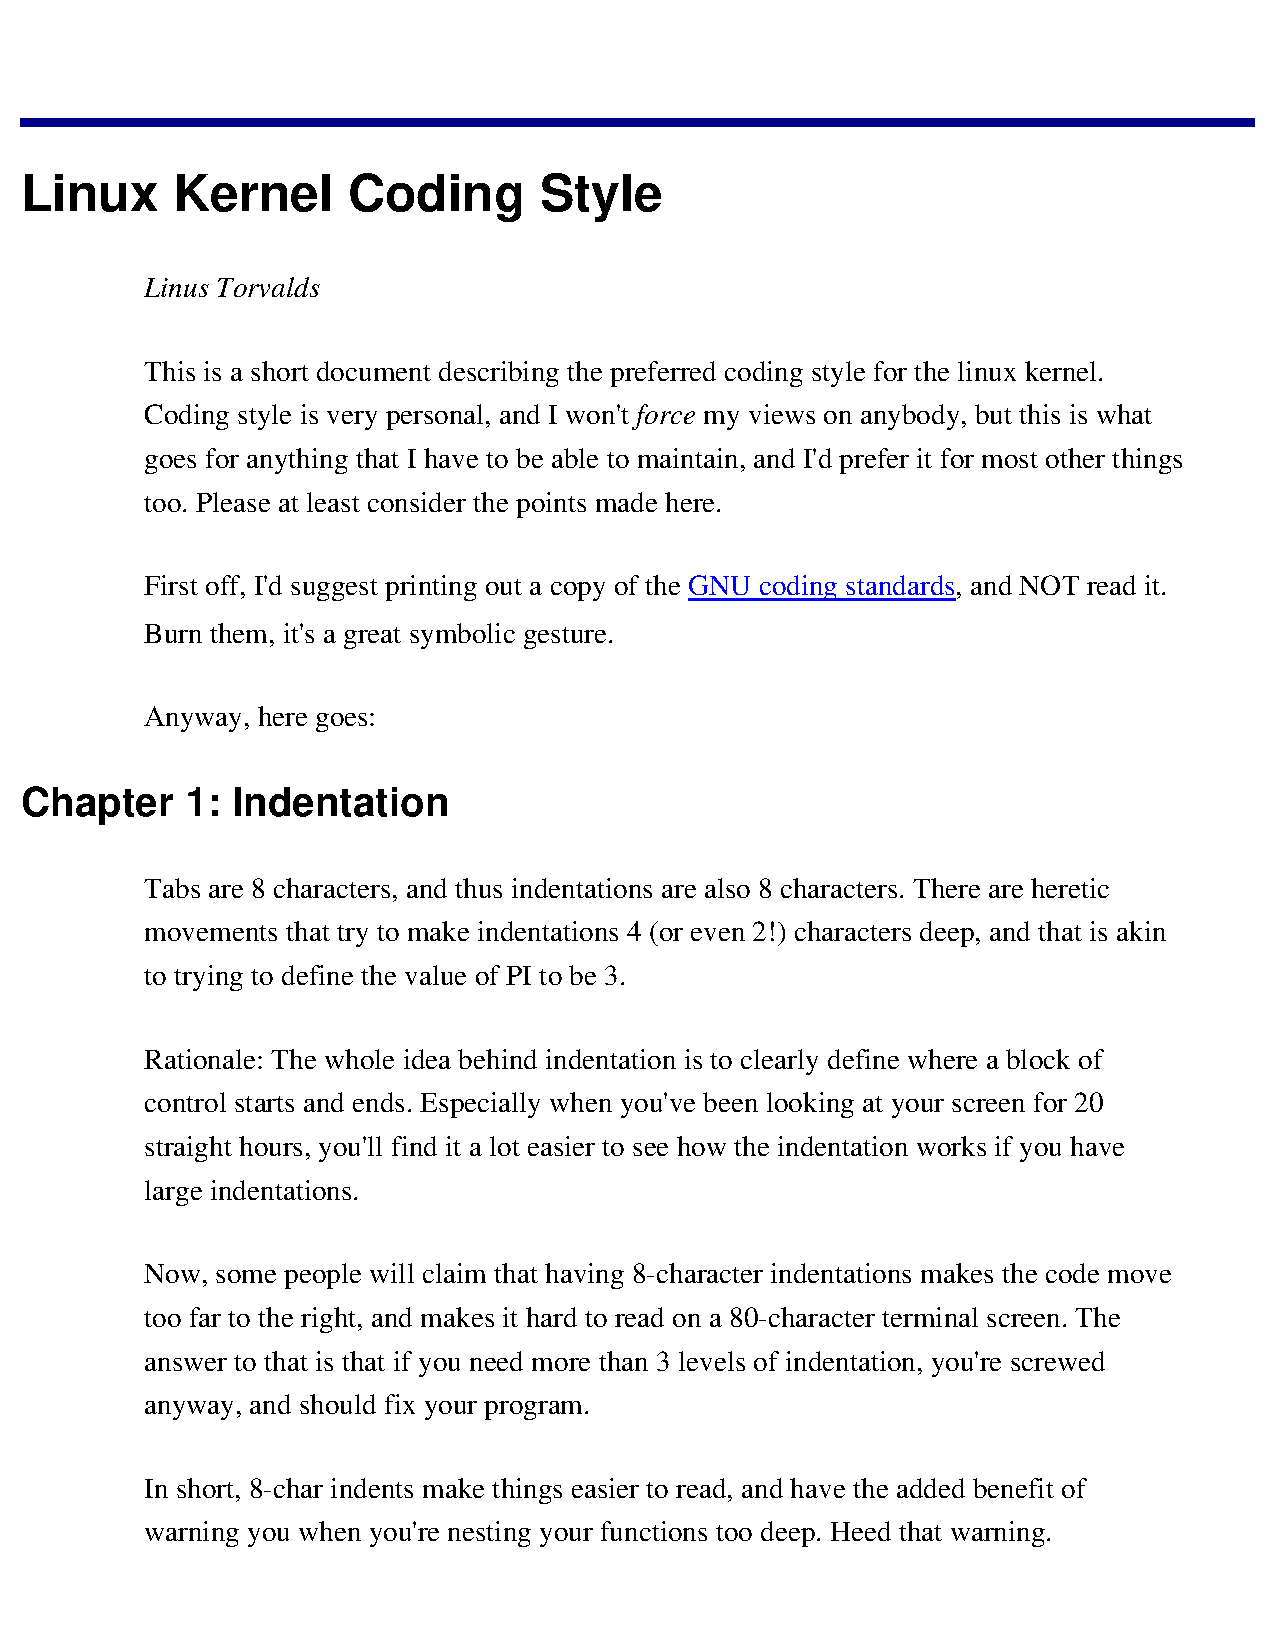
\includegraphics[page=1, width=1\textwidth]{kernelstyle.pdf}
    \end{figure}
    \newpage

    \section{GNU Coding Standards}
    Link zum ganzen Dokument
    \href{http://www.gnu.org/prep/standards/}{GNU Coding Standards}
    \begin{figure}[h!]
    \includegraphics[page=5, width=1\textwidth]{gnustandard.pdf}
    \end{figure}
\end{appendix}

\end{document}

